\section{A Metric for Quantifying the Safety of Soft Robots}
Thereafter, we propose a quantitative safety metric for \emph{blunt} contacts~\citep{haddadin2011safe} between soft robots and humans that captures the particular characteristics that continuum soft robots exhibit (e.g., elasticity, actuation through their structure, Cosserat rod dynamics, etc.).
Importantly, the presented safety metric fulfills all the mandatory requirements that we laid out previously. % (e.g., based on a soft robotic dynamical model, computationally tractable, differentiable, etc.).
First, we state the necessary background on soft robotic dynamics and contact models. Subsequently, we derive the dynamics of a collision between the continuum soft robot and the human (body part).
Next, we propose two flavors of the safety metric: (i) the \glsxtrfull{SRISC} captures the injury risk for a \emph{given} contact geometry, soft robot state, and actuation sequence. We envision this criterion to be useful for control applications with safety guarantees.
The second flavor, (ii) the \glsxtrfull{SRDHC}, captures the inherent safety of an integrated soft robot design (e.g., also considering the control policy) and leverages the \gls{SRISC} for estimating the maximum injury risk over all possible contact geometries, feasible robot states, and actuation sequences.
Apart from the procedure for formulating this safety metric, one of the key innovations here is that we identify a closed-form solution to the collision dynamics, which renders the computation of the \gls{SRISC} to be computationally tractable.

\subsection{Background on Soft Robot Dynamics and Contact Model}
Following the Cosserat rod theory, we can capture the kinematic behavior of slender structures such as continuum soft robots by considering the deformations of the robot's backbone. As the 1D spatial deformations of this backbone are still an infinite-dimensional problem, the field has developed many methods, such as \gls{PCC}~\citep{webster2010design}, \gls{PCS}~\citep{renda2018discrete}, and \gls{GVS}~\citep{renda2020geometric}, to describe such deformations with a finite number of finite vectors of configuration variables $q \in \mathbb{R}^n$. The associated forward kinematic model then allows us to define the geometric positional Jacobian $J_\mathrm{p}(q, s) \in \mathbb{R}^{3 \times n}$, where $s \in (0,L]$ is the backbone abscissa/coordinate and $L$ is the length of the entire continuum structure.
Independent of the specific chosen kinematic model, the \gls{EOM} of a continuum soft robot can often be stated as~\citep{armanini2023soft, della2023model}
\begin{equation}\label{eq:safetymetric:soft_robot_configuration_space_dynamics}
    M(q) \, \ddot{q} + C(q, \dot{q}) \, \dot{q} + \partial_{q} \, \mathcal{U}(q) + D \, \dot{q} = A(q) \, \tau + \tau_\mathrm{c},
\end{equation}
$M(q) \in \mathbb{R}^{n \times n}$ and $C(q, \dot{q}) \in \mathbb{R}^{n \times n}$ consider the inertial and Coriolis effects of the soft robot system, respectively.
$\partial_{q} \, \mathcal{U}(q) \in \mathbb{R}^n$ captures the forces stemming from the potential $\mathcal{U}(q): \mathbb{R}^n \to \mathbb{R}$.
Often times, the potential forces simplify to $\partial_{q} \, \mathcal{U}(q) =  G(q) + K q$, where $G(q) \in \mathbb{R}^{n}$ describes the gravitational forces, and $K \succ 0 \in \mathbb{R}^{n \times n}$ is the stiffness matrix.
Dissipation is integrated through the damping matrix $D \succ 0 \in \mathbb{R}^{n \times n}$.
$\tau(t,q,\dot{q}) \in \mathbb{R}^{m}$ contributes the actuation (determined by a control policy) that acts through the linear map $A(q) \in \mathbb{R}^{n \times m}$ on the generalized coordinates.

The term $\tau_\mathrm{c} \in \mathbb{R}^n$ collects all contributions by external contact forces on the generalized coordinates.
In the following, we will assume that the soft robot is only in contact with the human at one discrete point and that only pure forces are reflected between the bodies during the contact (i.e., no Cartesian torques).
Specifically, we assume that the contact occurs at the backbone abscissa $s_\mathrm{c} \in (0, L]$ and that the contact exhibits a constant surface normal of $n_\mathrm{c} \in \mathcal{S}^3$ which is a unit vector and, with that, $\mathcal{S}^3 = \{ n_\mathrm{c} \in \mathbb{R}^3: \lVert n_\mathrm{c} \rVert_2 = 1 \}$.
We now describe with $\delta_\mathrm{c} > 0$ a penetration between the soft robot and the soft tissue of the human.
Then, the generalized torque acting on the soft robot as a consequence of the contact is given by $\tau_\mathrm{c} = -J^\top(q,s_\mathrm{c}) \, n_\mathrm{c} \, f_\mathrm{c}(\delta_\mathrm{c}, \dot{\delta}_\mathrm{c}) = -J_\mathrm{c}^\top(q, s_\mathrm{c}, n_\mathrm{c}) \, f_\mathrm{c}(\delta_\mathrm{c}, \dot{\delta}_\mathrm{c})$, where $f_\mathrm{c}(\delta_\mathrm{c}, \dot{\delta}_\mathrm{c}) \in \mathbb{R}_{\geq 0}$ is the scalar non-negative contact force.
In the following, we will frequently omit the dependency of symbols, such as $J_\mathrm{c}(q)$, on the $(s_\mathrm{c}, n_\mathrm{c})$ to simplify the notation.
While the formulation that we use in this chapter for formulating the safety metric is compatible with many of the contact models that have been studied in the literature, such as Hunt-Crossley~\citep{hunt1975coefficient, aouaj2021predicting}, Hertz~\citep{johnson1987contact, park2011designing, she2020comparative}, etc., we will mainly focus in the following on a linear spring-damper contact model~\citep{iso2016collaborative, haddadin2009requirements} given by
\begin{equation}
    f_\mathrm{c}(\delta_\mathrm{c}, \dot{\delta}_\mathrm{c}) =
    \begin{cases}
        0 & \delta_\mathrm{c} \leq 0,\\
        k_\mathrm{c} \, \delta_\mathrm{c} + d_\mathrm{c} \, \dot{\delta}_\mathrm{c} & \delta_\mathrm{c} > 0,\\
    \end{cases}
\end{equation}
where $k_\mathrm{c} \in \mathbb{R}_{>0}$ is the contact stiffness and $d_\mathrm{c} \in \mathbb{R}_{\geq 0}$ is the contact damping coefficient.
If we assume the soft robot surface material and the human soft tissue to have spring constants and damping coefficients of $k_\mathrm{R,surf}$, $k_\mathrm{H,st}$, and $d_\mathrm{R}$, $d_\mathrm{H}$, respectively, then we can connect the spring-dampers in series
\begin{equation}
    k_\mathrm{c} = \left (\frac{1}{k_\mathrm{R,surf}} + \frac{1}{k_\mathrm{H,st}} \right )^{-1},
    \qquad
    d_\mathrm{c} = \left (\frac{1}{d_\mathrm{R}} + \frac{1}{d_\mathrm{H}} \right )^{-1}.
\end{equation}
Please note that the effective spring constant of many human body parts is reported in ISO/TS 15066:2016~\citep{iso2016collaborative}.

\subsection{Collision Dynamics}
We now progress towards a formulation of the collision dynamics as motions of the soft robot and the human body part along the contact surface normal $n_\mathrm{c}$.

First, we describe the motion of the contact point of the soft robot with position and velocity $x_\mathrm{R}, \dot{x}_\mathrm{R} \in \mathbb{R}$.
We can project the dynamics of \eqref{eq:safetymetric:soft_robot_configuration_space_dynamics} into this 1D motion through the expression $\dot{x}_\mathrm{R} = J_\mathrm{c} \, \dot{q}$ yielding the form~\citep{khatib1987unified, della2019exact, della2020model, stolzle2024guiding}
\begin{equation}
    \Lambda_\mathrm{c}(q) \, \Ddot{x}_\mathrm{R} + \eta_\mathrm{c}(q,\dot{q}) \, \dot{x}_\mathrm{R} + J_\mathrm{c,M}^{+\top}(q) ( \partial_{q} \, \mathcal{U}(q) + D \dot{q} ) = J_\mathrm{c,M}^{+\top}(q) \, A(q) \, \tau - f_{\mathrm{c}}(\delta_\mathrm{c}, \dot{\delta}_\mathrm{c}),
\end{equation}
where $J_\mathrm{c,M}^{+\top}(q, s_\mathrm{c},n_\mathrm{c}) = M^{-1}J_\mathrm{c}^\top(J_\mathrm{c} M^{-1} J_\mathrm{c}^\top)^{-1} \in \mathbb{R}^{n \times 1}$ is the dynamically consistent pseudo-inverse, $\Lambda_\mathrm{c}(q, s_\mathrm{c},n_\mathrm{c}) = (J_\mathrm{c} \, M^{-1} J_\mathrm{c}^\top)^{-1} \in \mathbb{R}^{1 \times 1}$ is the reflected inertia of the soft robot at the contact point~\citep{haddadin2009requirements, iso2016collaborative}, and $\eta_\mathrm{c}(q,\dot{q},s_\mathrm{c},n_\mathrm{c}) = \Lambda_\mathrm{c}(q) \, (J_\mathrm{c} M^{-1} C - \dot{J}_\mathrm{c}) \in \mathbb{R}^{1 \times n}$ collects the Cartesian Coriolis and centrifugal terms~\citep{khatib1987unified}.
As mentioned already previously, if not explicitly stated otherwise, we will in the following, to simplify the notation, drop the specific dependency on the contact geometry $(s_\mathrm{c}, n_\mathrm{c})$: $J_\mathrm{c,M}^{+\top}(q) = J_\mathrm{c,M}^{+\top}(q,s_\mathrm{c},n_\mathrm{c})$, $\Lambda_\mathrm{c}(q) = \Lambda_\mathrm{c}(q,s_\mathrm{c},n_\mathrm{c})$, etc.

Next, we move towards modeling the behavior of the human body part. In literature, the human body part is usually modeled as a point mass\footnote{Please note that the effective mass of various human body parts is reported in ISO/TS 15066:2016~\citep{iso2016collaborative}.} $m_\mathrm{H}$~\citep{haddadin2011safe, iso2016collaborative} that moves in 1D along the surface normal of the contact with state $(x_\mathrm{H},\dot{x}_\mathrm{H})$. Instead, we take here a conservative approach and assume that the human body is constrained in its motion with velocity $v_\mathrm{H} \in \mathbb{R}$ towards the soft robots (i.e., $m_\mathrm{H} \gg \Lambda(q) \: \forall q$). This represents the \emph{worst case}.
After the coordinate change $\delta_\mathrm{c}(t) = x_\mathrm{R}(t) - x_\mathrm{H}$, $\dot{\delta}_\mathrm{c} = \dot{x}_\mathrm{R}(t) + v_\mathrm{H}$, % where $x^{\mathrm{c}0} \in \mathbb{R}$ is the position of the initial contact, 
where $x_\mathrm{H} \in \mathbb{R}$ is the position of the soft tissue surface, and while only considering the case of contact (i.e., $\delta_\mathrm{c} \geq 0$), the collision dynamics are given by
\begin{equation}
    \Lambda_\mathrm{c}(q) \, \Ddot{\delta}_\mathrm{c} + \eta_\mathrm{c}(q,\dot{q}) \, \dot{\delta}_\mathrm{c} + J_\mathrm{c,M}^{+\top}(q) ( \partial_{q} \, \mathcal{U}(q) + D \dot{q} ) = J_\mathrm{c,M}^{+\top}(q) \, A(q) \, \tau - k_\mathrm{c} \, \delta_\mathrm{c} - d_\mathrm{c} \, \dot{\delta}_\mathrm{c}.
\end{equation}
We are now interested in identifying the maximum force $f_\mathrm{c}(t)$ that occurs during the entire time of the contact.
Therefore, we can neglect any damping forces, such as $d_\mathrm{c} \, \dot{\delta}_\mathrm{c}$ and $D \, \dot{q}$, as they dissipate energy, and, therefore, reduce the maximum contact force.
Furthermore, we assume that the Coriolis effects are sufficiently small and can be neglected as well.
Finally, we assume that the change of configuration during the collision is sufficiently small such that the dynamic matrices can be approximated as constant: 
\begin{equation}\label{eq:safetymetric:constant_reflected_inertia_and_actuation_matrix_definition}
    m_\mathrm{R} = \Lambda_\mathrm{c}(q_{\mathrm{c}}^0) \approx \Lambda_\mathrm{c}(q),
    \qquad
    A_\mathrm{c} = J_\mathrm{c,M}^{+\top}(q_{\mathrm{c}}^0) \, A(q_{\mathrm{c}}^0) \approx J_\mathrm{c,M}^{+\top}(q) \, A(q),
    \quad
    \forall \: t \geq t_\mathrm{c}^0,
\end{equation}
where the $q_{\mathrm{c}}^0$ is the configuration of the robot at the beginning of the contact.
The same assumption also allows us to linearize the potential forces of the soft robot with 
\begin{equation}\label{eq:safetymetric:collision_potential_forces}
    f_{\mathcal{U}} = J_\mathrm{c,M}^{+\top}(q) \, \partial_{q} \, \mathcal{U}(q) \approx \underbrace{J_\mathrm{c,M}^{+\top}(q_{\mathrm{c}}^0) \, \partial_{q} \, \mathcal{U}(q_{\mathrm{c}}^0)}_{f_{\mathcal{U}}^{\mathrm{c}0}} + \underbrace{\frac{\partial}{\partial q} J_\mathrm{c,M}^{+\top}(q) \, \partial_{q} \, \mathcal{U}(q) \Big |_{q=q_{\mathrm{c}}^0} \,  J_\mathrm{c,M}^{+}(q_{\mathrm{c}}^0)}_{k_\mathrm{R}}  \, \delta_\mathrm{c},
\end{equation}
where $k_\mathrm{R} \in \mathbb{R}$ is the local stiffness of the system against small perturbations and $f_{\mathcal{U}}^{\mathrm{c}0}$ are the potential forces present at the start of the contact.
Furthermore, we assume the actuation force to be constant, which can be easily accomplished by conservatively considering the maximum actuation force $f_\tau = \max_t \left | A_\mathrm{c} \, \tau(t) \right |$ that the robot experiences during the collision.
Integrating the stated assumptions into the \gls{EOM} results in the approximated collision dynamics (during contact)
\begin{equation}\label{eq:safetymetric:simplified_collision_dynamics}
    m_\mathrm{R} \, \Ddot{\delta}_\mathrm{c} + (k_\mathrm{R} + k_\mathrm{c}) \, \delta_\mathrm{c} = f_\tau - f_{\mathcal{U}}^{\mathrm{c}0}.
\end{equation}
To avoid computationally expensive simulations of the collision, we identify a closed-form solution to the collision dynamics
\begin{equation}\small\label{eq:safetymetric:collision_dynamics_cfs}
\begin{split}
    \delta_\mathrm{c}(t) =& \: \left (\delta_\mathrm{c}^0-\frac{f_\tau-f_{\mathcal{U}}^{\mathrm{c}0}}{k_\mathrm{R} + k_\mathrm{c}} \right ) \cos \left ( \sqrt{\frac{k_\mathrm{R} + k_\mathrm{c}}{m_\mathrm{R}}} \, t \right ) + \dot{\delta}_\mathrm{c}^0 \sqrt{\frac{m_\mathrm{R}}{k_\mathrm{R} + k_\mathrm{c}}} \, \sin \left ( \sqrt{\frac{k_\mathrm{R} + k_\mathrm{c}}{m_\mathrm{R}}} \, t \right ) + \frac{f_\tau-f_{\mathcal{U}}^{\mathrm{c}0}}{k_\mathrm{R} + k_\mathrm{c}},\\
    \dot{\delta}_\mathrm{c}(t) =& \: -\sqrt{\frac{k_\mathrm{R} + k_\mathrm{c}}{m_\mathrm{R}}} \left (\delta_\mathrm{c}^0 - \frac{f_\tau-f_{\mathcal{U}}^{\mathrm{c}0}}{k_\mathrm{R} + k_\mathrm{c}} \right ) \, \sin \left ( \sqrt{\frac{k_\mathrm{R} + k_\mathrm{c}}{m_\mathrm{R}}} \, t \right ) + \dot{\delta}_\mathrm{c}^0 \, \cos \left ( \sqrt{\frac{k_\mathrm{R} + k_\mathrm{c}}{m_\mathrm{R}}} \, t \right ),
\end{split}
\end{equation}
where we assume without loss of generality that $t_\mathrm{c}^0=0$ at the start of the collision, and $\delta_\mathrm{c}^0$ is the initial penetration depth, although generally $\delta_\mathrm{c}^0 = 0$.
The initial penetration velocity can be computed as a function of the configuration-space velocity as $\dot{\delta}_\mathrm{c}^0 = J_\mathrm{c}(q_{\mathrm{c}}^0) \, \dot{q}_{\mathrm{c}}^0 + v_\mathrm{H}$.

\begin{figure}[h!]
    \centering
    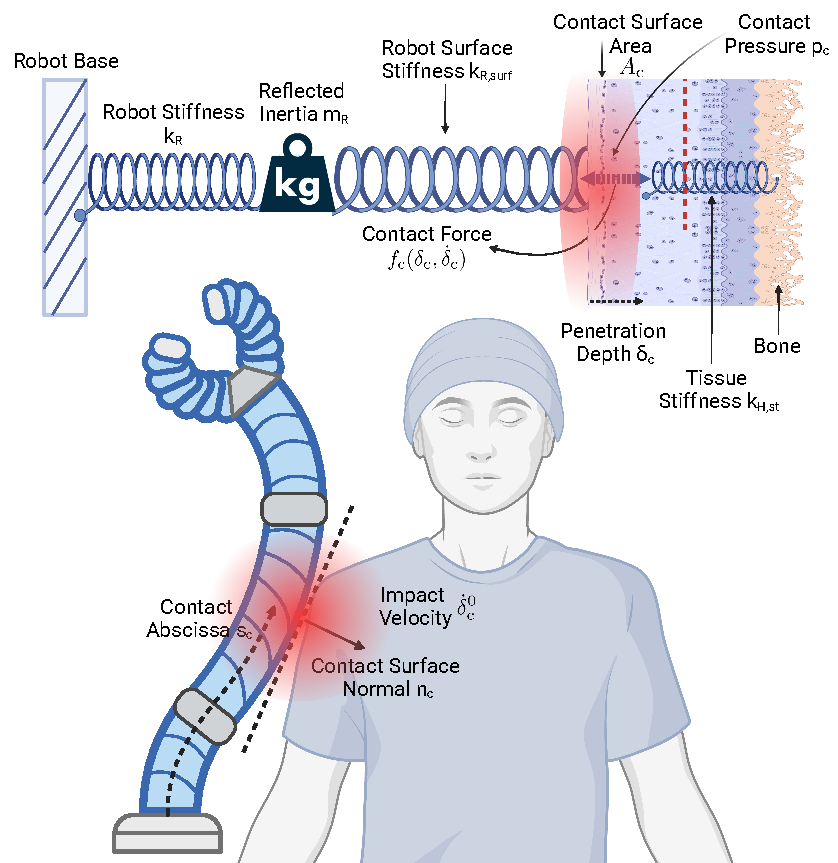
\includegraphics[width=0.65\linewidth]{safetymetric/figures/injury_severity_criterion.pdf}
    \caption{Proposed \glsxtrfull{SRISC} as a safety criterion for soft robots: The maximum contact pressure/stress $\max_t p_\mathrm{c}(t) = \max_t \frac{f_\mathrm{c}(t)}{A_\mathrm{c}}$ experienced during the (potential) collision acts as a proxy for the expected injury risk~\citep{iso2016collaborative}, where $f_\mathrm{c}(t)$ denotes the contact force and $A_\mathrm{c}$ the contact area. For computing $f_\mathrm{c}(t)$, we derive the dynamics of the collision (i.e., the time evolution of the penetration depth $\delta_\mathrm{c}(t)$) by projecting the dynamics of the soft robot onto a 1D Cartesian motion along the contact surface normal. In order to get a conservative estimate of the injury risk, we assume the human body part to be constrained in its motion (i.e., that the inertia of the human body part dominates the reflected inertia of the soft robot $m_\mathrm{R}$).}
    \label{fig:safetymetric:injury_severity_criterion_illustration}
\end{figure}

\subsection{Soft Robot Injury Severity Criterion}
Following the standards established in ISO/TS 15066:2016~\citep{iso2016collaborative}, we consider the maximum contact pressure, also sometimes referred to as stress~\citep{haddadin2009requirements}, experienced during the collision as a proxy for the injury risk. Therefore, we define the \gls{SRISC} for a given tuple $(q_{\mathrm{c}}^0,s_\mathrm{c}, n_\mathrm{c})$ capturing the contact geometry as
\begin{equation}
    \mathrm{SRISC}(q_{\mathrm{c}}^0,\dot{\delta}_\mathrm{c}^0,\tau,s_\mathrm{c},n_\mathrm{c}) = \max_t p_\mathrm{c} = \max_t \frac{f_\mathrm{c}(t)}{A_\mathrm{c}(t)} \leq \frac{\max_t f_\mathrm{c}(t)}{\min_t A_\mathrm{c}(t)} =  \frac{k_\mathrm{c} \max_t \delta_\mathrm{c}(t)}{\min_t A_\mathrm{c}(t)},
\end{equation}
where $p_\mathrm{c}(t)$ is the contact pressure/stress, and $A_\mathrm{c}$ is the contact area. We illustrate the derivation and definition of the \gls{SRISC} in Fig.~\ref{fig:safetymetric:injury_severity_criterion_illustration}.

The closed-form solution to the collision dynamics of \eqref{eq:safetymetric:collision_dynamics_cfs} allows us to upper-bound the maximum contact force $\max_t f_\mathrm{c}(t)$ that is encountered during the collision as
\begin{equation}\label{eq:safetymetric:maximum_contact_force_closed_form}
     \max_{t}f_\mathrm{c}(t) = k_\mathrm{c} \, \left ( \frac{f_\tau-f_{\mathcal{U}}^{\mathrm{c}0}}{k_\mathrm{R} + k_\mathrm{c}} + \sqrt{\left ( \delta_\mathrm{c}^0 - \frac{f_\tau-f_{\mathcal{U}}^{\mathrm{c}0}}{k_\mathrm{R} + k_\mathrm{c}} \right )^2 + \left (\dot{\delta}_\mathrm{c}^0 \right )^2 \frac{m_\mathrm{R}}{k_\mathrm{R} + k_\mathrm{c}} } \right ).
\end{equation}

\begin{figure}[ht]
    \centering
    \subfigure[Penetration depth $\delta_\mathrm{c}(t)$]{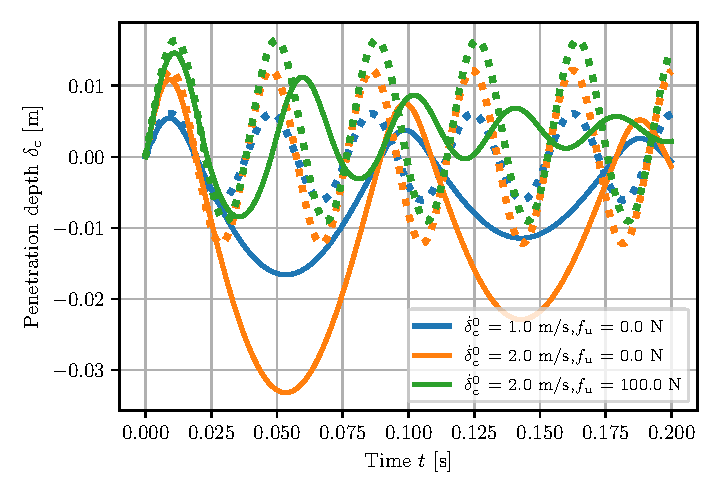
\includegraphics[width=0.49\linewidth, trim={5, 5, 5, 5}]{safetymetric/figures/closed_form_solution_verification/penetration_depth_vs_time.pdf}}
    \subfigure[Penetration velocity $\dot{\delta}_\mathrm{c}(t)$]{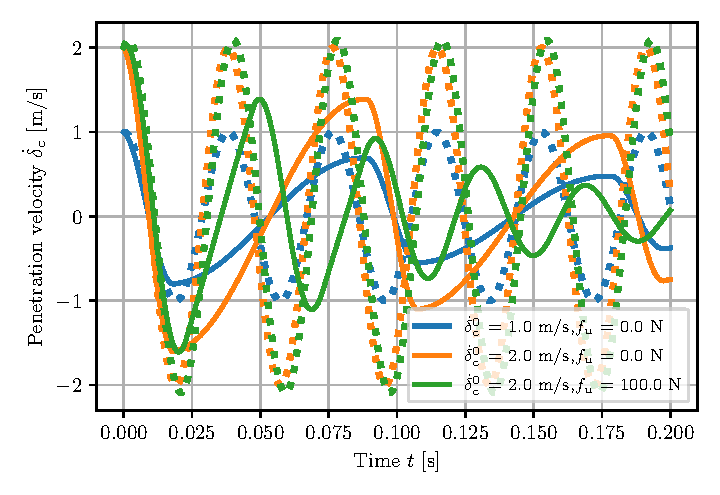
\includegraphics[width=0.49\linewidth, trim={5, 5, 5, 5}]{safetymetric/figures/closed_form_solution_verification/penetration_velocity_vs_time.pdf}}\\
    \subfigure[Contact force $f_\mathrm{c}(t)$]{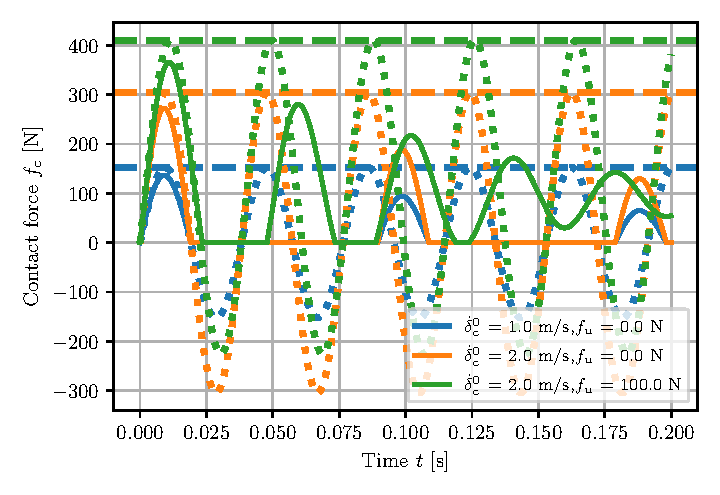
\includegraphics[width=0.5\linewidth, trim={5, 5, 5, 5}]{safetymetric/figures/closed_form_solution_verification/contact_force_vs_time.pdf}}
    \caption{
        Verification of closed-form solution to \eqref{eq:safetymetric:simplified_collision_dynamics}: The solid lines represent numerical integrations of the hybrid dynamics 
        $m_\mathrm{R} \, \Ddot{\delta}_\mathrm{c} + k_\mathrm{R} \, \delta_\mathrm{c} + d_\mathrm{R} \, \dot{\delta}_\mathrm{c} + f_\mathrm{c}(\delta_\mathrm{c}) = f_\tau - f_{\mathcal{U}}^{\mathrm{c}0}$ with $f_\mathrm{c}(\delta_\mathrm{c}) = k_\mathrm{c} \, \delta_\mathrm{c} + d_\mathrm{c} \, \dot{\delta}_\mathrm{c} \: \forall \, \delta_\mathrm{c} > 0$ and $f_\mathrm{c}(\delta_\mathrm{c}) = 0 \: \forall \; \delta_\mathrm{c} \leq 0$. 
        The dotted lines represent the closed-form solution to the time evolution reported in \eqref{eq:safetymetric:collision_dynamics_cfs} based on the dynamics in \eqref{eq:safetymetric:simplified_collision_dynamics} that describe the behavior during the contact phase. The dashed lines represent the (conservative) maximum contact force that could be encountered during the collision as determined by the closed-form expression \eqref{eq:safetymetric:maximum_contact_force_closed_form}. 
        As system parameters, we choose $m_\mathrm{R} = \SI{1}{kg}$, $k_\mathrm{R} = \SI{2}{kN \per m}$, $d_\mathrm{R} = \SI{4}{Ns \per m}$, $k_\mathrm{c} = \SI{25}{kN \per m}$, which represents the spring constant of the human chest according to ISO/TS 15066:2016~\citep{iso2016collaborative}, $d_\mathrm{c} = \SI{20}{Ns \per m}$, and $\delta_\mathrm{c}^0 = \SI{0}{m}$.
        Please note that in all case we assume $f_{\mathcal{U}}^{\mathrm{c}0} = 0$ and $v_\mathrm{H} = 0$.
    }
    \label{fig:safetymetric:closed_form_solution_verification}
\end{figure}

We verify and visualize the behavior of the closed-form expression from \eqref{eq:safetymetric:collision_dynamics_cfs} and its upper bound \eqref{eq:safetymetric:maximum_contact_force_closed_form} in Fig.~\ref{fig:safetymetric:closed_form_solution_verification}. It can be clearly seen how \eqref{eq:safetymetric:maximum_contact_force_closed_form} represents a conservative upper bound on the actual contact forces the system experiences if we were to also account for the hybrid nature of the dynamics and the damping of the system.

\begin{figure}[ht!]
    \centering
    \subfigure[Initial deflection $q_\mathrm{c}^0$ vs. Robot stiffness $k_\mathrm{R}$]{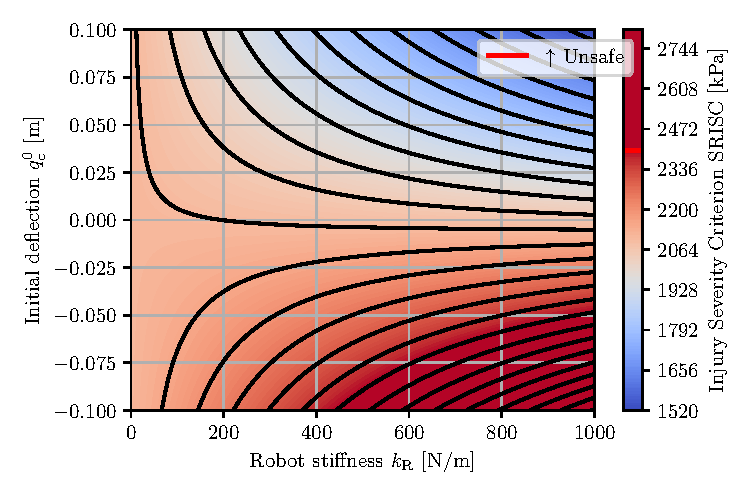
\includegraphics[width=0.49\linewidth, trim={5, 5, 5, 5}]{safetymetric/figures/mass_spring_robot/robot_stiffness_vs_initial_deflection.pdf}\label{fig:safetymetric:mass_spring_robot_characterization:robot_stiffness_vs_initial_deflection}}
    \subfigure[Contact stiffness $k_\mathrm{c}$ vs. robot stiffness $k_\mathrm{R}$]{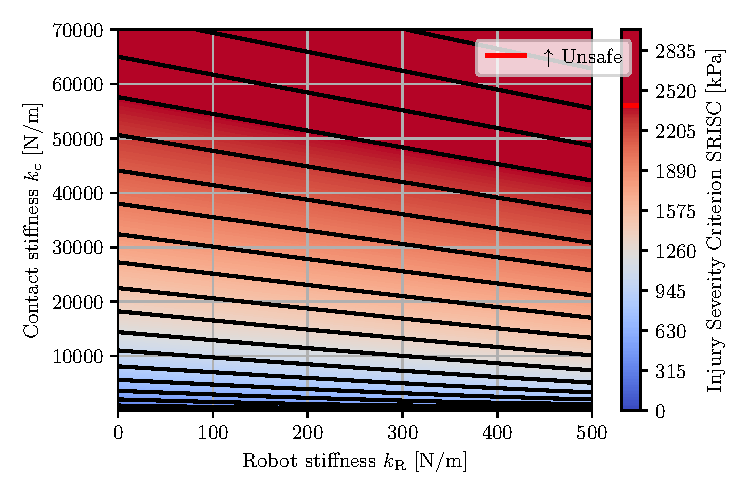
\includegraphics[width=0.49\linewidth, trim={5, 5, 5, 5}]{safetymetric/figures/mass_spring_robot/robot_stiffness_vs_contact_stiffness.pdf}\label{fig:safetymetric:mass_spring_robot_characterization:contact_stiffness_vs_robot_stiffness}}
    \\ \vspace{-0.2cm}
    \subfigure[Initial velocity $\dot{q}_\mathrm{c}^0$ vs. robot mass $m_\mathrm{R}$]{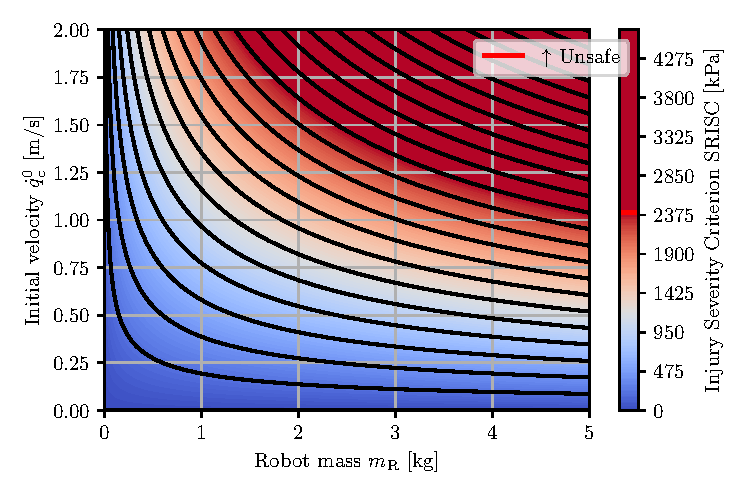
\includegraphics[width=0.49\linewidth, trim={5, 5, 5, 5}]{safetymetric/figures/mass_spring_robot/robot_mass_vs_initial_velocity.pdf}\label{fig:safetymetric:mass_spring_robot_characterization:robot_mass_vs_initial_velocity}}
    \vspace{-0.2cm}
    \caption{Characterization of the \gls{SRISC} on the mass-spring robot example.
        Here, we (closely) consider the collision between the mass-spring robot and the human chest. Therefore, if we conservatively assume the robot surface to be rigid, the spring constant of the contact with the chest is given as $k_\mathrm{c} = k_\mathrm{H} = \SI{25}{kN \per m}$. Furthermore, we assume a contact area of $\SI{1.5}{cm^2}$, an external force of $u=\SI{0}{N}$, and a equilibrium position of $q^0 = \SI{0}{m}$. Finally, according to ISO/TS 15066:2016~\citep{iso2016collaborative}, the maximum acceptable contact pressure/stress in transient conditions is given as $\SI{2400}{kPa}$, which serves as our threshold on the maximum acceptable \gls{SRISC}.
        \textbf{Panel~(a):} Evaluating the influence of robot stiffness $k_\mathrm{R}$ and the deflection of the soft robot at the beginning of the collision $q_\mathrm{c}^0$ on the \gls{SRISC}. We choose $m_\mathrm{R} = \SI{1}{kg}$ and $\dot{q}_\mathrm{c}^0 = \SI{2}{m/s}$.
        \textbf{Panel~(b):} Evaluating the influence of contact stiffness $k_\mathrm{c}$ and the robot stiffness $k_\mathrm{R}$ on the \gls{SRISC}. We choose $m_\mathrm{R} = \SI{1}{kg}$, $q_\mathrm{c}^0 = -\SI{0.1}{m}$, and $\dot{q}_\mathrm{c}^0 = -\SI{1.5}{m/s}$.
        \textbf{Panel~(c):} Evaluating the influence of robot mass $m_\mathrm{R}$ and the robot velocity at the beginning of the collision $\dot{q}_\mathrm{c}^0$ on the \gls{SRISC}. We choose $k_\mathrm{R} = \SI{1}{kN \per m}$ and $q_\mathrm{c}^0 = \SI{0}{m}$.
    }
    \label{fig:safetymetric:mass_spring_robot_characterization}
    \vspace{-0.2cm}
\end{figure}

\subsubsection{Example: Mass-Spring Robot}
First, we consider the most \emph{basic} soft robot - a damped mass-spring system with dynamics 
\begin{equation}
    m_\mathrm{R} \, \ddot{q} + k_\mathrm{R} \, (q-q^0) + d_\mathrm{R} \, \dot{q} = u + f_\mathrm{c},
\end{equation}
where $q \in \mathbb{R}$ and $q^0 \in \mathbb{R}$ is the equilibrium extension. 
Assuming $\delta_\mathrm{c}(t) = q(t)$ (i.e., the robot is in contact with the human when $q \geq 0$) and $v_\mathrm{H} = 0$, the \gls{SRISC} is then given by
\begin{equation}
     \mathrm{SRISC} = \frac{k_\mathrm{c}}{A_\mathrm{c}} \, \left (\frac{u - k_\mathrm{R} (q_{\mathrm{c}}^0 - q^0)}{k_\mathrm{R} + k_\mathrm{c}} + \sqrt{\left ( \frac{u - k_\mathrm{R} (q_{\mathrm{c}}^0 - q^0)}{k_\mathrm{R} + k_\mathrm{c}} \right )^2 + \left (\dot{q}_\mathrm{c}^0 \right )^2 \frac{m_\mathrm{R}}{k_\mathrm{R} + k_\mathrm{c}} } \right ),
\end{equation}
where $q_{\mathrm{c}}^0$ is the mass-spring position at which the collision starts and $\dot{q}_\mathrm{c}^0$ is the associated velocity.

Here, the \gls{SRISC} exhibits the limits
\begin{equation}
    \lim_{k_\mathrm{R} \to 0, u \to 0} \mathrm{SRISC} = \frac{\sqrt{m_\mathrm{R} \, k_\mathrm{c}}}{A_\mathrm{c}} \, \dot{q}_\mathrm{c}^0,
    \qquad
    \lim_{k_\mathrm{R} \to \infty} \mathrm{SRISC} = \frac{k_\mathrm{c}}{A_\mathrm{c}} \, \left ( - (q_{\mathrm{c}}^0 - q^0 ) + \left | q_{\mathrm{c}}^0 - q^0 \right | \right ).
\end{equation}
If $q_{\mathrm{c}}^0 \geq q^0$, which can be interpreted as the spring being in its equilibrium or stretched at the beginning of the collision, then the limit $k_\mathrm{R} \to \infty$ simplifies to $\lim_{k_\mathrm{R} \to \infty} \mathrm{SRISC} = 0$.

We characterize the \gls{SRISC} for this mass-spring robot example in the case of a collision with a human chest and present the results in Fig.~\ref{fig:safetymetric:mass_spring_robot_characterization}. 
Fig.~\ref{fig:safetymetric:mass_spring_robot_characterization:robot_stiffness_vs_initial_deflection} allows us to analyze what influence the robot stiffness has on the \gls{SRISC}: In the limit of $k_\mathrm{R} \to 0$ with $u = 0$, the contact pressure is solely influenced by the robot's initial velocity $\dot{q}_\mathrm{c}^0$, its mass $m_\mathrm{R}$, and the contact stiffness $k_\mathrm{c}$. However, as $k_\mathrm{R} > 0$, we can notice a bifurcation behavior: if the robot is stretched at the beginning of the collision (i.e., $q_\mathrm{c}^0 > 0$), then the contact stress \gls{SRISC} is decreased as $k_\mathrm{R}$ is increased. Oppositely, if the robot is compressed at the beginning of the collision (i.e., $q_\mathrm{c}^0 < 0$), then the contact stress \gls{SRISC} is increased as $k_\mathrm{R}$ is increased.
Fig.~\ref{fig:safetymetric:mass_spring_robot_characterization:contact_stiffness_vs_robot_stiffness} shows, as expected, that increasing the contact stiffness leads to a higher peak contact pressure.
Analog to the known results in the realm of rigid robotics~\citep{haddadin2009requirements, haddadin2013towards}, it can be easily seen in Fig.~\ref{fig:safetymetric:mass_spring_robot_characterization:robot_mass_vs_initial_velocity} how higher velocities and higher robot masses/inertia lead to higher injury severities and safety risks.
This analysis allows us to draw two important takeaways: (1) it is crucial to consider the maximum deformation of the soft robot we would expect to occur during operation to assess its safety, (2) as the robot's stiffness is increased, the \emph{worst-case} injury severity is also increased~\citep{abidi2017intrinsic} - confirming the intuition of how soft robots with their material softness and lower inertia exhibit a more compliant behavior than traditional rigid robots.

\begin{figure}[ht]
    \centering
    \subfigure[Contact backbone coordinate $s_\mathrm{c}$ vs. polar angle $\theta_\mathrm{c}$]{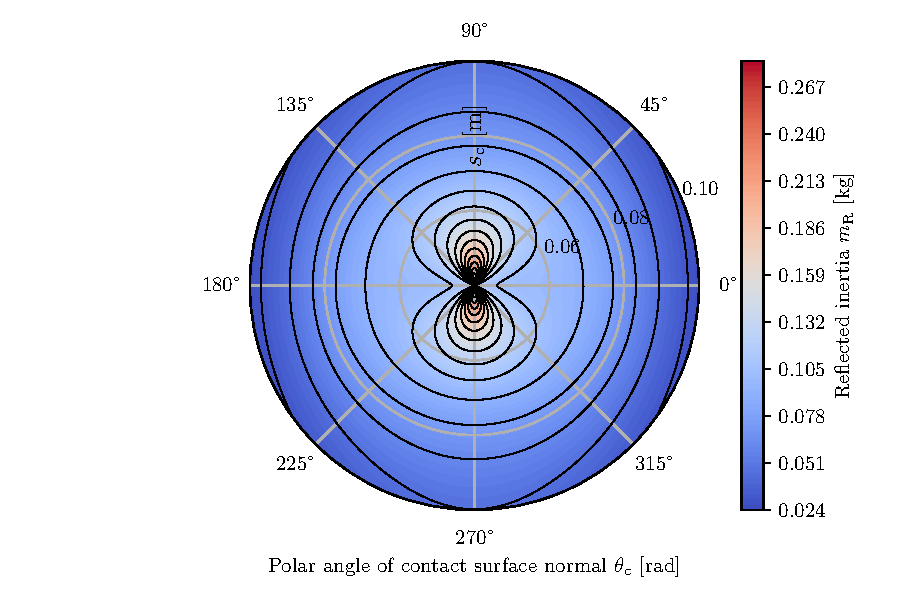
\includegraphics[width=0.43\linewidth, trim={5, 5, 5, 5}]{safetymetric/figures/planar_cs_reflected_inertia_characterization/planar_cs_reflected_inertia_for_theta_vs_s_c_cropped.pdf}}
    \subfigure[Bending strain $\kappa_\mathrm{be}$ vs. axial strain $\sigma_\mathrm{ax}$]{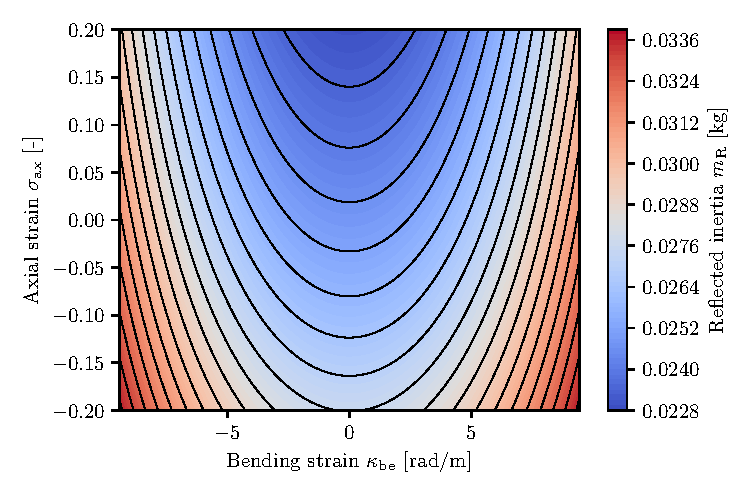
\includegraphics[width=0.56\linewidth, trim={5, 5, 5, 5}]{safetymetric/figures/planar_cs_reflected_inertia_characterization/planar_cs_reflected_inertia_for_kappa_be_vs_sigma_ax.pdf}}
    \caption{Characterization of the reflected inertia, also called effective mass~\citep{haddadin2009requirements, kirschner2021notion}, on the example of a planar \gls{CS} soft robot. 
    \textbf{Left:} Variation of the collision backbone coordinate $s_\mathrm{c}$ against the polar angle of contact $\theta_\mathrm{c}$, where $\theta_\mathrm{c} = 0$ corresponds to a perpendicular collision with the backbone and $n_\mathrm{c} = (1, 0)$ and $\theta_\mathrm{c} = \frac{\pi}{2}$ relates to a parallel collision with the robot backbone and $n_\mathrm{c} = (0,1)$. We assume here a soft robot in its equilibrium configuration (i.e., $q = 0_3$).
    \textbf{Right:} Variation of the bending strain $\kappa_\mathrm{be}$ and the axial strain $\sigma_\mathrm{ax}$ for a perpendicular collision ($n_\mathrm{c} = (0,1)$) at the distal end of the robot ($s_\mathrm{c} = \SI{0.1}{m}$).
    }
    \label{fig:safetymetric:planar_cs_reflected_inertia_characterization}
    \vspace{-0.2cm}
\end{figure}

\begin{figure}[ht]
    \centering
    \subfigure[Contact backbone coordinate $s_\mathrm{c}$ vs. polar angle $\theta_\mathrm{c}$]{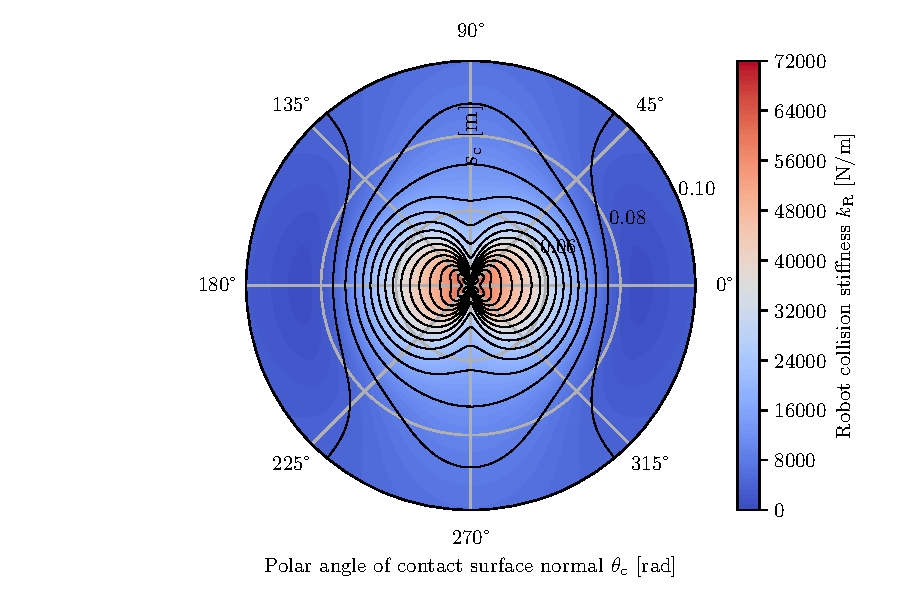
\includegraphics[width=0.49\linewidth]{safetymetric/figures/planar_cs_robot_collision_stiffness_characterization/planar_cs_robot_collision_stiffness_for_theta_c_vs_s_c_cropped.pdf}\label{fig:safetymetric:planar_cs_robot_collision_stiffness_characterization:theta_c_vs_s_c}}
    \subfigure[Bending strain $\kappa_\mathrm{be}$ vs. contact polar angle $\theta_\mathrm{c}$]{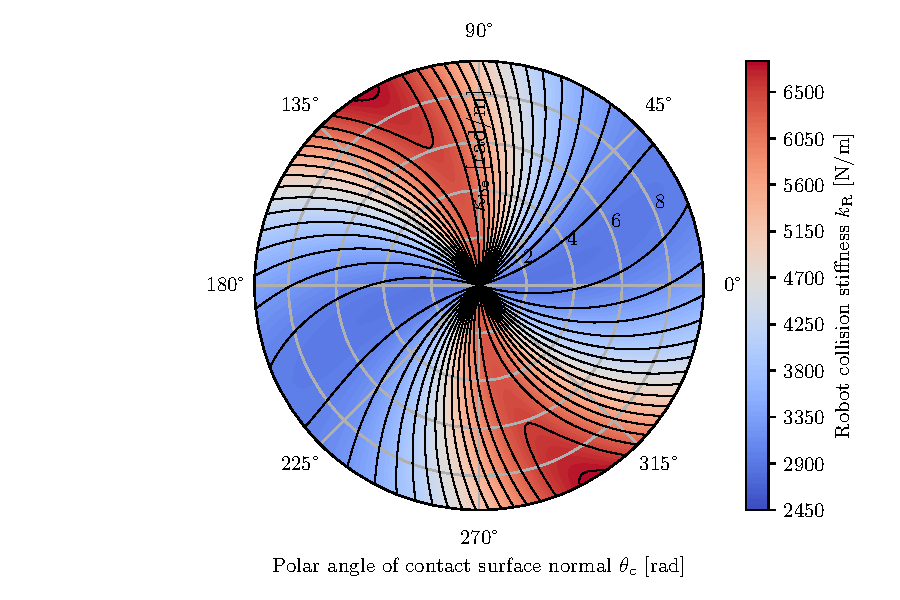
\includegraphics[width=0.49\linewidth]{safetymetric/figures/planar_cs_robot_collision_stiffness_characterization/planar_cs_robot_collision_stiffness_for_theta_c_vs_kappa_be_cropped.pdf}\label{fig:safetymetric:planar_cs_robot_collision_stiffness_characterization:theta_c_vs_kappa_be}}
    \caption{Characterization of the local robot collision stiffness $k_\mathrm{R}$ vs. polar angle $\theta_\mathrm{c}$ on the example of a planar \gls{CS} soft robot.
    \textbf{Left:} Variation of the collision backbone coordinate $s_\mathrm{c}$ against the polar angle of contact $\theta_\mathrm{c}$, where $\theta_\mathrm{c} = 0$ corresponds to a perpendicular collision with the backbone and $n_\mathrm{c} = (1, 0)$ and $\theta_\mathrm{c} = \frac{\pi}{2}$ relates to a parallel collision with the robot backbone and $n_\mathrm{c} = (0,1)$. We assume here a soft robot in its equilibrium configuration (i.e., $q = 0_3$).
    \textbf{Right:} Variation of the bending strain $\kappa_\mathrm{be}$ against the polar angle of contact $\theta_\mathrm{c}$ at the distal end of the robot ($s_\mathrm{c} = \SI{0.1}{m}$).
    }
    \label{fig:safetymetric:planar_cs_robot_collision_stiffness_characterization}
\end{figure}

\subsubsection{Example: Planar Piecewise Constant Strain Robot}
% 1 Figure giving an example how the contact location influences the injury severity.
% \begin{itemize}
%     \item Variation of injury severity for various contact geometries (e.g., various locations along the backbone, various contact surface normal) and configurations.
%     \item Variation across model discretization granularity.
% \end{itemize}

We now consider a planar $N$ segment \gls{PCS} robot, as introduced in Chapter~\ref{chp:background}. Here, the configuration of the $i$th segment is characterized by its spatially constant strain $\xi_i = \begin{bmatrix}
    \kappa_{\mathrm{be},i} & \sigma_{\mathrm{sh},i} & \sigma_{\mathrm{ax},i}
\end{bmatrix}^\top$, where $\kappa_{\mathrm{be},i}$ is the bending, $\sigma_{\mathrm{sh},i}$ the shear, and $\sigma_{\mathrm{ax},i}$ the axial/elongation strain~\citep{renda2018discrete}.
The collision dynamics are then given as
\begin{equation}
    \Lambda_\mathrm{c}(q) \, \Ddot{\delta}_\mathrm{c} + \eta_\mathrm{c}(q,\dot{q}) \, \dot{\delta}_\mathrm{c} + J_\mathrm{c,M}^{+\top}(q) ( G(q) + S \, q + D \dot{q} ) = J_\mathrm{c,M}^{+\top}(q) \, A(q) \, \tau - k_\mathrm{c} \, \delta_\mathrm{c} - d_\mathrm{c} \, \dot{\delta}_\mathrm{c},
\end{equation}
where $S \in \mathbb{R}^{3N \times 3N}$ is the linear stiffness of the robot, $G(q) \in \mathbb{R}^{3N}$ captures the gravitational forces, and $\tau \in \mathbb{R}^m$ represents the actuator forces.
We build the JAX~\citep{jax2018github} implementation of these dynamics on the \emph{JSRM}\footnote{\url{https://github.com/tud-phi/jax-soft-robot-modelling}} package~\citep{stolzle2024experimental}.

As we have seen in the previous example of the mass-spring robot, two of the variables that have the largest impact on the \gls{SRISC} are the reflected inertia $m_\mathrm{R}$, as defined in
\eqref{eq:safetymetric:constant_reflected_inertia_and_actuation_matrix_definition}, and the local soft robot stiffness in the collision direction $k_\mathrm{R}$, as defined in \eqref{eq:safetymetric:collision_potential_forces}.
Therefore, we present in Figures \ref{fig:safetymetric:planar_cs_reflected_inertia_characterization} \& \ref{fig:safetymetric:planar_cs_robot_collision_stiffness_characterization} a characterization of the reflected inertia $m_\mathrm{R}$ and the local robot stiffness $k_\mathrm{R}$, respectively.
In both cases, we consider a planar \gls{CS} segment (i.e., $N=1$) that has a length of $\SI{0.1}{m}$, a radius of \SI{0.02}{m}, a material density of \SI{1070}{kg \per m^3}, an elastic modulus of $E=\SI{0.5}{MPa}$ and a shear modulus of $G=\SI{0.2}{MPa}$.
The results show that the reflected inertia is highest at the proximal end of the robot/segment (i.e., $s_\mathrm{c} \to 0$) and for collisions that are parallel to the backbone, which, for our definition of our coordinate system with the soft robot in its straight configuration aligned with the y-axis, means that $\theta_\mathrm{c} = \frac{\pi}{2} + \pi \, n$ and $n_\mathrm{c} = \begin{bmatrix}
    0 & \pm 1
\end{bmatrix}^\top$. Furthermore, when considering perpendicular collisions with the backbone, the inertia increases with the bending strain and a compressed backbone (i.e., an increase in mass density).
Concerning the robot collision stiffness, we find that it is highest at the proximal end of the soft robot. At the distal end, we identify larger stiffnesses for parallel collisions, although the exact characteristics will depend on the choice of backbone radius/second moment of area. With increased bending strain, the polar angle with the highest stiffness will also change, as seen in Fig.~\ref{fig:safetymetric:planar_cs_robot_collision_stiffness_characterization:theta_c_vs_kappa_be}.

\begin{figure}[ht!]
    \centering
    \subfigure[Bending strain velocity $\dot{\kappa}_\mathrm{be}$ vs. mass density $\rho$]{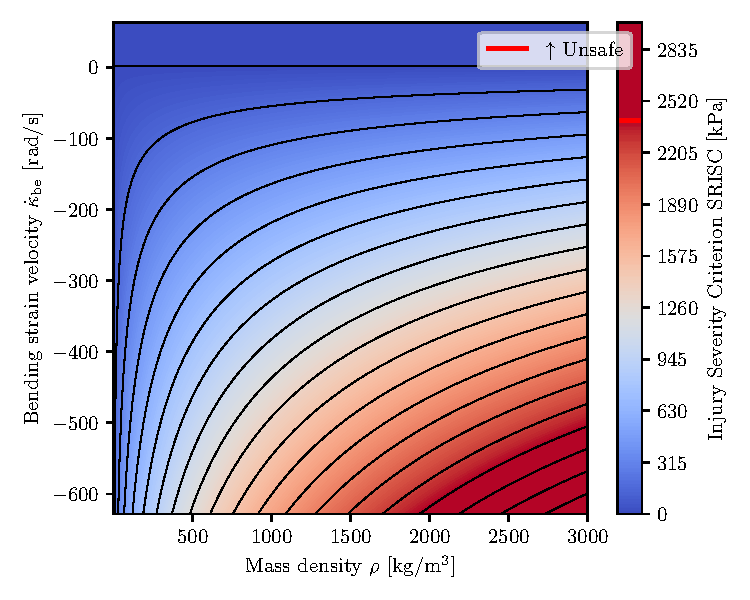
\includegraphics[width=0.49\linewidth]{safetymetric/figures/planar_cs_injury_severity_criterion/planar_cs_isc_for_bending_strain_velocity_vs_mass_density.pdf}\label{fig:safetymetric:planar_cs_injury_severity_criterion:bending_strain_velocity_vs_mass_density}}
    \subfigure[Robot length $L$ vs. backbone coordinate $s_\mathrm{c}$]{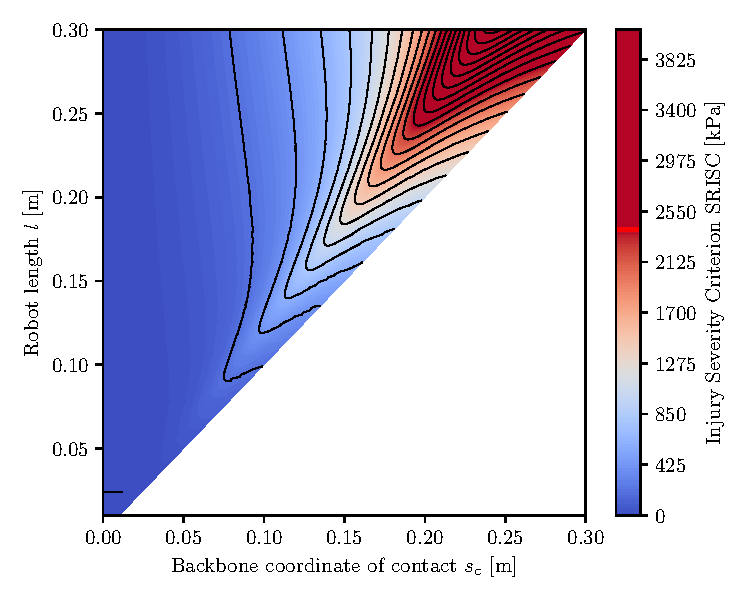
\includegraphics[width=0.49\linewidth]{safetymetric/figures/planar_cs_injury_severity_criterion/planar_cs_isc_robot_length_vs_s_c.pdf}\label{fig:safetymetric:planar_cs_injury_severity_criterion:robot_length_vs_s_c}}
    \\
    \subfigure[Contact backbone coordinate $s_\mathrm{c}$ vs. polar angle $\theta_\mathrm{c}$]{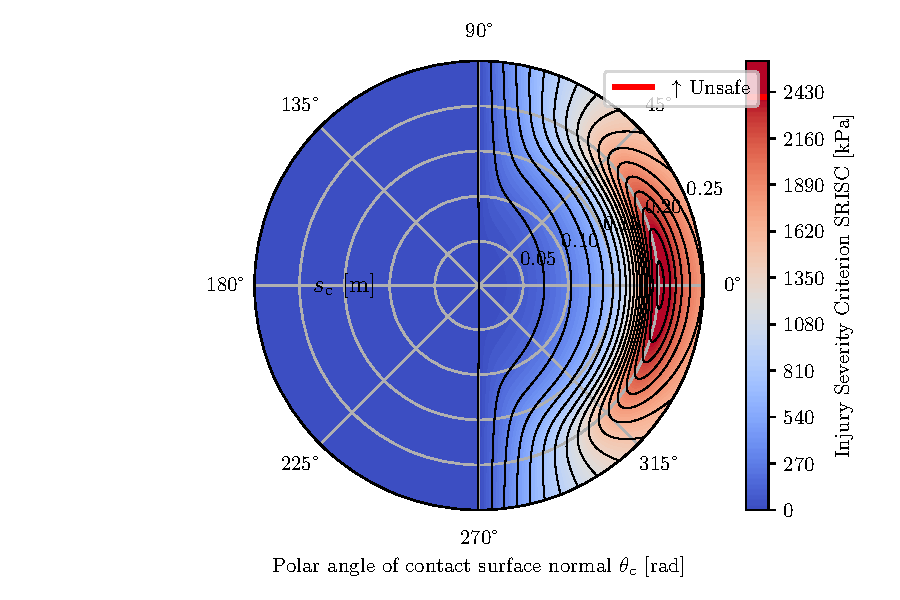
\includegraphics[width=0.49\linewidth]{safetymetric/figures/planar_cs_injury_severity_criterion/planar_cs_isc_for_theta_c_vs_s_c_cropped.pdf}\label{fig:safetymetric:planar_cs_injury_severity_criterion:theta_c_vs_s_c}}
    \subfigure[Bending strain $\kappa_\mathrm{be}$ vs. polar angle $\theta_\mathrm{c}$]{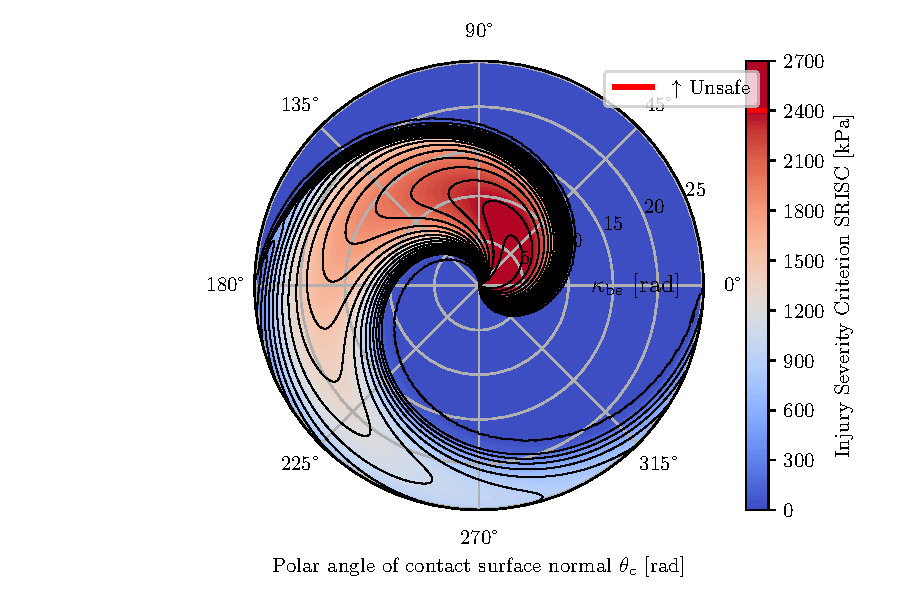
\includegraphics[width=0.49\linewidth]{safetymetric/figures/planar_cs_injury_severity_criterion/planar_cs_isc_for_theta_c_vs_kappa_be_cropped.pdf}\label{fig:safetymetric:planar_cs_injury_severity_criterion:theta_c_vs_kappa_be}}
    \caption{Characterization of the \gls{SRISC} on a planar \gls{CS} robot.
    \textbf{Panel~(a):} Variation of the robot's mass density $\rho$ and the bending strain velocity $\dot{\kappa}_\mathrm{be}$. We assume a perpendicular collision ($n_\mathrm{c} = (1,0)$) at the tip of the segment ($s_\mathrm{c} = \SI{0.25}{m}$).
    \textbf{Panel~(b):} Variation of the total robot length $L$ and the backbone coordinate $s_\mathrm{c}$ where the collision occurs. We assume a perpendicular collision ($n_\mathrm{c} = (1,0)$) with a soft robot in its equilibrium configuration (i.e., $q=0_3$).
    \textbf{Panel~(c):} Variation of the backbone coordinate $s_\mathrm{c}$ against the polar angle $\theta_\mathrm{c}$ of the contact surface where the collision occurs. Here, $\theta_\mathrm{c} = 0$ corresponds to a surface normal of $n_\mathrm{c} = (1,0)$ and $\theta_\mathrm{c} = \frac{\pi}{2}$ to $n_\mathrm{c} = (0,1)$. The soft robot is assumed to be in its equilibrium configuration (i.e., $q=0_3$).
    \textbf{Panel~(d):} Variation of the bending strain $\kappa_\mathrm{be}$ against the polar angle $\theta_\mathrm{c}$ of the contact surface where the collision occurs. We assume a collision with the distal end of the soft robot (i.e., $s_\mathrm{c} = \SI{0.25}{m}$).
    }
    \label{fig:safetymetric:planar_cs_injury_severity_criterion}
\end{figure}

In Fig.~\ref{fig:safetymetric:planar_cs_injury_severity_criterion}, we characterize the behavior of the \gls{SRISC} on the case of a planar \gls{CS} soft robot with a nominal robot length $L = \SI{0.25}{m}$, a backbone radius of $R = \SI{0.02}{m}$, a nominal mass density of $\rho = \SI{1070}{kg \per m^3}$, an elastic modulus of $E = \SI{0.5}{MPa}$, a shear modulus of $G = \SI{0.2}{MPa}$, a contact area of $A_\mathrm{c} = \SI{1.5}{cm^2}$, the spring constant of the human chest $k_\mathrm{H,st} = \SI{25}{kN \per m}$, and a soft robot surface material stiffness of $k_{\mathrm{R,surf}} = \SI{7.5}{kN \per m}$.
In all cases, we set the external forcing to $f_\tau = 0_3$, consider the human to be stationary and constrained with $v_\mathrm{H} = \SI{0}{m \per s}$, and assume a maximum threshold of \SI{2400}{kPa} on the \gls{SRISC}, which mirrors the maximum transient contact stress that is acceptable for collisions with the chest sternum according to ISO/TS 15066:2016~\citep{iso2016collaborative}.
% In Fig.~\ref{fig:safetymetric:planar_cs_injury_severity_criterion:bending_strain_velocity_vs_mass_density}, we can observe that, as expected, the maximum contact stress, and with that, the \gls{SRISC}, increases with mass density and a larger bending velocity in the direction of the collision.
% The results shown in Fig.~\ref{fig:safetymetric:planar_cs_injury_severity_criterion:robot_length_vs_s_c} are very interesting: while the \gls{SRISC} increases with an increased length of the segment, which is not too unexpected as longer soft robots exhibit larger Cartesian space velocities for the same strain-space velocities, we observe the the maximum contract stress is usually not at the tip of the distal end of the robot, but instead at at roughly \SI{75}{\percent} of its length. We hypothesize that the underlying reason is that some quantities, such as stiffness and reflected inertia, are at their maximum at the proximal end, while other quantities - in particular the Cartesian velocity - are at their maximum and the distal end leading the global maximum of the \gls{SRISC} to be in between proximal and distal end.
% Fig.~\ref{fig:safetymetric:planar_cs_injury_severity_criterion:theta_c_vs_s_c} exhibits the same characteristics while the polar angle with the maximum contact stress will always depend on the velocities and actuation that are applied to the soft robot.
% Finally, we observe in Fig.~\ref{fig:safetymetric:planar_cs_injury_severity_criterion:theta_c_vs_kappa_be} the maximum \gls{SRISC} to be at a straight backbone configuration with the \gls{SRISC} decreasing with an increased bending strain.
In Fig.\ref{fig:safetymetric:planar_cs_injury_severity_criterion:bending_strain_velocity_vs_mass_density}, we see that, as expected, the maximum contact stress—and therefore the \gls{SRISC}—rises with increased mass density and higher bending velocity in the collision direction. The results in Fig.~\ref{fig:safetymetric:planar_cs_injury_severity_criterion:robot_length_vs_s_c} are particularly intriguing: while the \gls{SRISC} increases with longer segment lengths—as longer soft robots exhibit higher Cartesian velocities for the same strain-space velocities—the maximum contact stress is typically not located at the very tip of the distal end but rather around \SI{75}{\percent} of the robot’s length. We hypothesize that this occurs because certain factors, such as stiffness and reflected inertia, peak at the proximal end, whereas others—especially Cartesian velocity—are maximized at the distal end, leading to an overall maximum \gls{SRISC} somewhere between the two. Similarly, Fig.~\ref{fig:safetymetric:planar_cs_injury_severity_criterion:theta_c_vs_s_c} displays analogous behavior, with the polar angle corresponding to the maximum contact stress varying based on the velocities and actuation applied to the soft robot. Finally, Fig.~\ref{fig:safetymetric:planar_cs_injury_severity_criterion:theta_c_vs_kappa_be} shows that the maximum \gls{SRISC} occurs at a straight backbone configuration, with the maximum \gls{SRISC} decreasing as bending strain increases.

\subsubsection{Example: Integrating a Control Policy}
% alternative heading: \subsection{Influence of Control Policy}
An important question when analyzing the safety of a closed-loop soft robotic system is what influence the control policy has on the \gls{SRISC}.
First, we consider a case where the behavior of the control policy $\tau(q,\dot{q})$ cannot be bounded or even inspected, such as it would be the case for controllers that contain integral terms or for many RL-based control policies.
In this case, access to actuation bounds $[\tau_\mathrm{min}, \tau_\mathrm{max}]$ provides us with the injury risk in the \emph{worst case scenario}.

Next, we consider the example of a \emph{PD+Feedforward}-like control structure that is relevant for many control policies that involve feedforward and/or feedback terms.
Specifically, we consider a fully-actuated setting (i.e., $n=m$) with an identity actuation matrix $A(q) = \mathbb{I}^n$.
Then, a regulator $\tau(q,\dot{q}) = \partial_{q} \, \mathcal{U}( q^\mathrm{d}) + K_\mathrm{p} \, (q^\mathrm{d}-q) - K_\mathrm{d} \, \dot{q}$ drives the system towards the setpoint $q^\mathrm{d}$~\citep{della2023model} and establishes the closed-loop dynamics
\begin{equation}
    M(q) \, \ddot{q} + C(q, \dot{q}) \, \dot{q} + \partial_{q} \, \mathcal{U}(q) + K_\mathrm{p} \, q + (D+K_\mathrm{d}) \, \dot{q} = \partial_{q} \, \mathcal{U}( q^\mathrm{d}) + K_\mathrm{p} \, q^\mathrm{d} + \tau_\mathrm{c},
\end{equation}
where $K_\mathrm{p}, K_\mathrm{d} \in \mathbb{R}^{n \times n}$ are the proportional and derivative feedback gains, respectively.
When re-formulating the simplified collision dynamics of \eqref{eq:safetymetric:simplified_collision_dynamics}, 
\begin{equation}
    m_\mathrm{R} \, \Ddot{\delta}_\mathrm{c} + (k_\mathrm{R} + k_\mathrm{c}) \, \delta_\mathrm{c} = J_\mathrm{c,M}^{+}(q_{\mathrm{c}}^0) \, (\partial_{q} \, \mathcal{U}(q^\mathrm{d}) +  K_\mathrm{p} \, q^\mathrm{d} - \partial_{q} \, \mathcal{U}(q_{\mathrm{c}}^0)).
\end{equation}
We notice that the feedforward control term acts through a constant force on the oscillatory system.
The proportional feedback term increases the local stiffness of the robot: $k_\mathrm{R} = \frac{\partial}{\partial q} J_\mathrm{c,M}^{+\top}(q) \, \left ( \partial_{q} \, \mathcal{U}(q) + K_\mathrm{p} \, q \right )\Big |_{q=q_{\mathrm{c}}^0} \,  J_\mathrm{c,M}^{+}(q_{\mathrm{c}}^0)$.
This analysis agrees with similar results known in literature~\citep{della2017controlling}.

\subsection{Soft Robot Design Hazardousness Criterion}
As presented in Fig.~\ref{fig:safetymetric:safety_metric_applications}, one application of a soft robotic safety metric would be to answer the question "\emph{How safe is this proposed soft robot design?}". The \gls{SRISC} on its own is not sufficient to answer this question as it relies on a knowledge of the soft robot state at the beginning of the collision $(q_{\mathrm{c}}^0, \dot{q}_{\mathrm{c}}^0)$, and the contact geometry $(s_\mathrm{c},n_\mathrm{c})$.
Therefore, we define the \gls{SRDHC} as the maximum injury severity that can be imposed by the soft robot over all feasible soft robot states, all possible contact geometries, and actuation sequences~\citep{wassink2007towards}
\begin{equation}
\begin{split}
    \mathrm{SRDHC} =& \: \max_{q \in \mathcal{Q}} \max_{\dot{\delta}_\mathrm{c}^0 \in [0,\dot{\delta}_\mathrm{c}^\mathrm{max}]} \max_{\tau \in [\tau_\mathrm{min}, \tau_\mathrm{max}]} \max_{s_\mathrm{c} \in (0,L]} \max_{n_\mathrm{c} \in \mathcal{S}^3} \mathrm{SRISC}(q_{\mathrm{c}}^0,\dot{\delta}_\mathrm{c}^0,\tau,s_\mathrm{c},n_\mathrm{c}),\\
    \leq& \: \max_{q \in \mathcal{Q}} \max_{s_\mathrm{c} \in (0,L]} \max_{n_\mathrm{c} \in \mathcal{S}^3} \mathrm{SRISC}(q_{\mathrm{c}}^0,\dot{\delta}_\mathrm{c}^\mathrm{max},\lVert \tau_\mathrm{max} \rVert_2,s_\mathrm{c},n_\mathrm{c}),
\end{split}
\end{equation}
where $\mathcal{Q}$ is the set of feasible soft robot configurations.
To make this optimization more tractable, we can leverage the stated upper bound with $\dot{\delta}_\mathrm{c}^\mathrm{max} = \lVert J_\mathrm{c} \rVert_2 \, \lVert \dot{q}_\mathrm{max} \rVert_2 + v_\mathrm{H}$
and $f_\tau^\mathrm{max} = \lVert A_\mathrm{c} \rVert_2 \, \lVert \max(|\tau_\mathrm{min}|,|\tau_\mathrm{max}|) \rVert_2$.
We note that the maximum value of $\dot{q}_\mathrm{max}$ that the robot can achieve autonomously is, in practice, often given by certain actuator characteristics (e.g., maximum servo velocity for tendon-driven actuation).

% We performed a preliminary investigation on the effect of the discretization on the estimated safety - and, in particular, the \gls{SRDHC}.
% The initial results reported in Fig.~\ref{fig:safetymetric:planar_pcs_design_hazardousness_criterion_discretization} show that approximating the soft robot with one or a few segments represents a conservative estimate of the actual safety - i.e., an overestimation of the injury severity. The underlying reason behind this behavior is that the actual soft robots can deform in infinite-dimensional space, while the approximation via the planar \gls{PCS} model limits the deformation modes and, with that, often increases the stiffness upon local contact. By increasing the discretization of the kinematic model underlying the safety metric, we can account for more deformation modes, and with that, reduce the overestimate of the injury severity.
We conducted a study to assess how discretization affects the estimated safety, with a particular focus on the \gls{SRDHC}. The initial results shown in Fig.~\ref{fig:safetymetric:planar_pcs_design_hazardousness_criterion_discretization} for varying the number of \gls{PCS} segments while keeping the robot length and all other system parameters constant indicate that approximating the soft robot with one or only a few segments leads to a conservative safety estimate—that is, an overestimation of the injury severity. This occurs because actual soft robots can deform in an infinite-dimensional space, whereas the planar \gls{PCS} model limits the available deformation modes and often increases the stiffness at the point of contact. By refining the discretization of the underlying kinematic model, we can capture more deformation modes and thereby reduce the overestimation of injury severity.

\begin{figure}
    \centering
    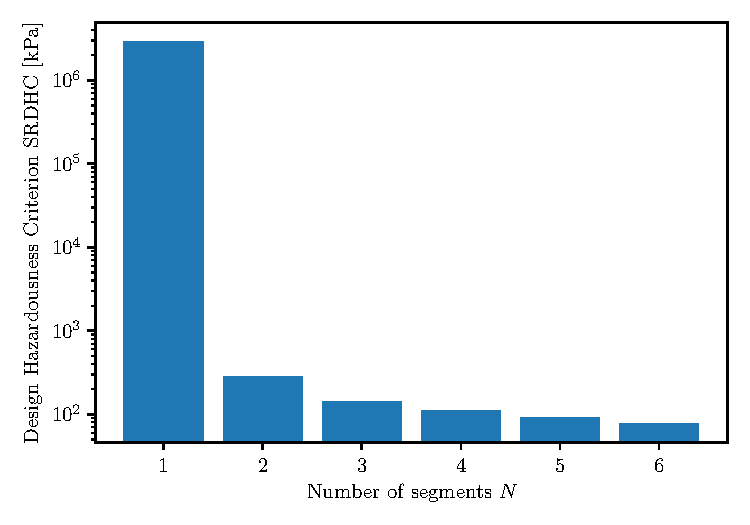
\includegraphics[width=0.5\linewidth]{safetymetric/figures/planar_pcs_design_hazardousness_criterion_discretization/design_hazardousness_criterion_bar_log.pdf}
    \caption{Analysis of the impact of varying the discretization of a planar \gls{PCS} robot on \gls{SRDHC} while keeping the total soft robot length constant at \SI{1}{m}.}
    \label{fig:safetymetric:planar_pcs_design_hazardousness_criterion_discretization}
\end{figure}